\documentclass[times, utf8, diplomski, numeric]{fer}
\usepackage[utf8]{inputenc}
\usepackage[T1]{fontenc}
\usepackage{currvita}
\usepackage{graphicx}
\usepackage{epstopdf}
\usepackage{listings}
\usepackage{textcomp}
\usepackage{booktabs}
\usepackage{algorithmic}
\usepackage{algorithm}
\usepackage{xfrac}
\usepackage[bookmarks]{hyperref}
\usepackage{color}

% koristimo zadebljane vektore, a ne strelice
\renewcommand{\vec}[1]{\mathbf{#1}}

% TODO komanda koja u PDFu daje crveni, kapitalizirani, bold text
\newcommand\todo[1]{\colorbox{yellow}{\textcolor{red}{#1}}}

% ovo je za numeriranje samo jedne linije unutar align okoline
\newcommand\numberthis{\addtocounter{equation}{1}\tag{\theequation}}

% definicija jezika koji nema nista, pa se nista ne naglasava
% koristi se za troadresni kod, ispise tokena i slicno
\lstdefinelanguage{blank}{
	sensitive=false, 
	morecomment=[l]{;},
}

% neke boje koje koristimo u formatiranju ispisa
\usepackage{color}
\definecolor{mygreen}{rgb}{0,0.6,0}
\definecolor{mylightgray}{rgb}{0.95,0.95,0.95}

% definicija formatiranja ispisa, ponesto promjenjena u odnosu na pretpostavljenu
\lstset{ %
  backgroundcolor=\color{mylightgray},   % choose the background color; you must add \usepackage{color} or \usepackage{xcolor}
  basicstyle=\footnotesize\ttfamily,        % the size of the fonts that are used for the code
  breakatwhitespace=false,         % sets if automatic breaks should only happen at whitespace
  breaklines=true,                 % sets automatic line breaking
  captionpos=b,                    % sets the caption-position to bottom
  commentstyle=\color{mygreen},    % comment style
  deletekeywords={...},            % if you want to delete keywords from the given language
  escapeinside={\%*}{*)},          % if you want to add LaTeX within your code
  extendedchars=true,              % lets you use non-ASCII characters; for 8-bits encodings only, does not work with UTF-8
  frame=none,                    % adds a frame around the code
  keepspaces=true,                 % keeps spaces in text, useful for keeping indentation of code (possibly needs columns=flexible)
  keywordstyle=\color{blue},       % keyword style
  language=c,           	       % the language of the code
  morekeywords={*,...},            % if you want to add more keywords to the set
  numbers=none,                    % where to put the line-numbers; possible values are (none, left, right)
  numbersep=5pt,                   % how far the line-numbers are from the code
  numberstyle=\tiny\color{gray}, % the style that is used for the line-numbers
  rulecolor=\color{black},         % if not set, the frame-color may be changed on line-breaks within not-black text (e.g. comments (green here))
  showspaces=false,                % show spaces everywhere adding particular underscores; it overrides 'showstringspaces'
  showstringspaces=false,          % underline spaces within strings only
  showtabs=false,                  % show tabs within strings adding particular underscores
  stepnumber=2,                    % the step between two line-numbers. If it's 1, each line will be numbered
  stringstyle=\color{red},     % string literal style
  tabsize=2,                       % sets default tabsize to 2 spaces
  title=\lstname                   % show the filename of files included with \lstinputlisting; also try caption instead of title
}

\begin{document}

\title{Jezični model temeljen na neuronskoj mreži}
\thesisnumber{1095}

\author{Florijan Stamenković}

\maketitle

\tableofcontents

\chapter{Uvod}


\chapter{Jezični model}

Jezični model jedan je od ključnih elemenata računalnog procesiranja prirodnog jezika. Glavni zadatak tom računalnom sustavu je ocjenjivanje pripadnosti teksta u prirodni jezik za koji je sustav rađen. Dodatno, poželjno je da sustav između više ponuđenih može izabrati tekst koji je najviše "u duhu" jezika. Primjerice, model hrvatskog jezika trebao bi biti sposoban ocijeniti da je niz \textit{"dan je lijep"} generalno više u duhu jezika od \textit{"lijepo dana biti"}, a da niz \textit{"it's a nice day"} u dotični jezik ne pripada.

Smislenost niza riječi može se promatrati iz pravopisne, gramatičke i semantičke perspektive. Dakle, model treba biti sposoban nizu \textit{"lijep dan"} dati bolju ocjenu nego nizu \textit{"ljep dan"}. Nadalje, treba bolje ocijeniti niz \textit{"lijep dan"} od niza \textit{"lijepo dani"}. Konačno, treba bolje ocijeniti niz \textit{"lijep dan"} od niza \textit{"staklen plan"}.

\section{Primjena}

Jezični modeli imaju velik broj primjena. Sustavi za strojno prevođenje koriste ih kako bi odabrali što smisleniji među više potencijalnih prijevoda. Sustavi za prepoznavanje govora koriste ih kako bi prepoznate slogove i riječi pretvorili u konačni tekst. Sustavi za pretraživanje teksta mogu ih koristiti za mjerenje sličnosti između termina pretrage i dokumenta. Ovo su samo neke od mnogih primjena, povećanjem dostupne količine informacija i mogućnosti njihove računalne obrade, moguće primjene i kvaliteta jezičnih modela imaju trend povećanja.

\section{Probabilistička definicija}

Pošto prirodni jezik omogućava praktično neiscrpne mogućnosti kombiniranja riječi u tekst, smisleno je jezični model razmatrati statistički. Na temelju što većeg korpusa teksta gradi se sustav koji za proizvoljni niz označava koliko je sličan tekstu iz korpusa. Kako bi se takav sustav izgradio, potrebno je smislenost teksta definirati probabilistički. Vjerojatnost niza riječi možemo zapisati na sljedeći način.

\[
P(\text{niz}) = P(w_1, w_2, ... , w_m)
\]

Pri tome je $P(w_1, w_2, ... , w_m)$ vjerojatnost slijeda od $m$ riječi u kojem je $i$-ta riječ upravo $w_i$. Tako definirana vjerojatnost može se faktorizirati.

\begin{align*}
P(w_1, w_2, ... , w_m)
  &= P(w_1) P(w_2 | w_1) P(w_3 | w_1, w_2) ... P(w_m | w_1, w_2, ... , w_{m - 1 }) \\
  &= \prod_{i = 1}^m{P(w_i|w_1, ... , w_{i - 1})}
\end{align*}

Pri tome je $P(w_i | w_1, ... , w_{i - 1})$ uvjetna vjerojatnost pojavljivanja riječi $w_i$ na $i$-toj poziciji u nizu, ako su joj prethodile riječi $w_1$, ... $w_{i - 1}$ na pozicijama $1$, ... , $i - 1$. Primjetimo kako je ovakva faktorizacija u skladu sa čovjekovim čitanjem teksta (slijedno po riječima).

Iako egzaktna, dobivena faktorizacija vjerojatnosti niza praktična jer je vjerojatnost riječi na poziciji $i$ uvjetovana svim prethodnim riječima. Pošto tekst može biti proizvoljne duljine, u jezičnim modelima se najčešće koristi kontekst ograničene duljine od $n$ riječi. Primjerice, za kontektst duljine $n = 3$, svaka riječ se razmatra samo s obzirom na prethodne dvije.

\begin{align*}
P(w_1, w_2, ... , w_m)
  &\approx P(w_1) P(w_2 | w_1) P(w_3 | w_1, w_2)  ... P(w_m | w_{m - 2}, w_{m - 1}) \\
  &\approx \prod_{i = 1}^m{P(w_i | w_{i - 2}, w_{i - 1})}
\end{align*}

Općenito, za proizvoljnu duljinu konteksta \textit{n} faktorizacija je sljedeća.

\begin{align*}
P(w_1, w_2, ... , w_m)
  &\approx P(w_1) P(w_2 | w_1) P(w_3 | w_1, w_2)  ... P(w_m | w_{m - (n - 1)}, w_{m - (n - 2)}, ... , w_{m - 1}) \\
  &\approx \prod_{i = 1}^m{P(w_i | w_{i - (n - 1)}, ... , w_{i - 1})}
\end{align*}

Ovakav jezični model više nije probabilistični egzaktan, ali se može puno lakše implementirati kao računalni sustav.

U nastavku ovog rada se slijed od \textit{n} riječi označava \textit{n}-gram. Za $n=1, 2, 3$ govorimo o "unigramu", "bigramu", odnosno "trigramu", dok za $n=4$ o "4-gramu" itd.

Kada se koristi ograničeni kontekst, javlja se pitanje optimalne duljine. S obzirom da na konačno značenje niza mogu utjecati riječi koje su od promatrane riječi proizvoljno daleko, može se pretpostaviti da je veći kontekst bolji od manjeg. Iako ovo u idealnom slučaju vrijedi, u praksi se koriste relativno male duljine konteksta, iz sljedećeg razloga. Vjerojatnost pojavljivanja nekog konkretnog niza riječi duljine $n$ pada eksponencijalno kako $n$ raste. Primjerice, ako promatramo bigrame, tada će se većina smislenih kombinacija od dvije riječi pojaviti u korpusu teksta na kojem se model bazira. U drugu ruku, ako razmatramo 100-grame, većina kombinacija od 100 riječi nikada se neće pojaviti u ograničenom korpusu teksta, što uključuje i smislene 100-grame. Kada se potom takav 100-gram pojavi pri korištenju modela na konkretnom zadatku, model će mu neopravdano pridjeliti vrlo malo vjerojatnost. U praksi se stoga često koriste konteksti duljine do četiri riječi, ovisno o primjeni. Modeli bazirani na velikom korpusu teksta mogu povećati kontekst do šest ili sedam riječi, rijetko više. 

Alternativni pristup ograničavanju veličine konteksta je kompresija odnosno aproksimacija konteksta pune duljine. Konkretno, ako kontekst prikažemo kao funkciju prethodnih riječi, moguća je sljedeća faktorizacija.

\begin{align*}
P(w_1, w_2, ... , w_m)
  &\approx P(w_1) P(w_2 | f(w_1)) P(w_3 | f(w_1, w_2)) ... P(w_m | f(w_1, w_2, ... , w_{n - 1 })) \\
  &\approx \prod_{i = 1}^n{P(w_i | f(w_1, ... , w_{i - 1}))}
\end{align*}

Pri tome funkcija $f(...)$ preslikava kontekst proizvoljne duljine u zapis fiksne duljine. Ovakva formulacija koristi se primjerice u izvedbi jezičnih modela korištenjem rekurzivnih neuronskih mreža. Pošto se u ovom radu ne koriste implementacije bazirane na toj formulaciji, neće se u ostatku teksta spominjati.

Postoje varijante jezičnih modela koje kao kontekst ne promatraju riječi koje doslovno prethode promatranoj, već riječi iz šire okoline. Neki modeli čak razmatraju "koncepte" sačinjene od nekoliko riječi koje se mogu pojaviti bilo gdje u tekstu. Ovakvi modeli se neće razmatrati u nastavku.

Konačno, bitno je spomenuti jezične modele bazirane na manjim lingvističkim jedinicama. Jezični modeli bazirani na morfemima i znakovima su od nedavno, pogotovo sa sve većom primjenom dubokih neuronskih mreža, postali uspooredivi i čak u nekim primjenama bolji od leksičkih modela.

\section{Načini izvedbe}

Postoje brojne implementacije jezičnih modela. Većina njih izvedena je iz probabilističke formulacije modela, ili tu formulaciju aproksimiraju. Tehnike korištene za izradu modela variraju. U ovom diplomskom radu biti će uspoređene izvedbe prebrojavanjem \textit{n}-grama, oblik neuronske mreže i log-bilinearni probabilistički model. Njihova definicija i opis slijede.

\chapter{Prebrojavanje \textit{n}-grama}

Najjednostavniji pristup implementaciji jezičnog modela bazira se na frekvenciji \textit{n}-grama. Definicija za uvjetnu vjerojatnost riječi baziranu na primjerice trigramima je sljedeća.

\[
P(w_i | w_{i - 2}, w_{i - 1}) = \frac{C(w_{i - 2}, w_{i - 1}, w_i)}{C(w_{i - 2}, w_{i - 1})}
\]

Pri tome je $C(w_a, ... , w_b)$ funkcija prebrojavanja koja za niz $w_a, ... , w_b$ daje broj njegovih pojavljivanja u korpusu teksta nad kojim se model gradi. Uvjetna vjerojatnost pojavljivanja riječi, s obzirom na prethodne dvije, je dakle broj pojavljivanja relevantnog trigrama, podjeljeno s brojem pojavljivanja bigrama koji joj prethode. Intuicija je sljedeća. Ako smo u tekstu obzervirali da se trigram \textit{"dan je lijep"} pojavljuje 10 puta, a bigram \textit{"dan je"} 12 puta, tada je $P("lijep" | "dan", "je") = 10 / 12$.

Ovako definiran procijenitelj vjerojatnosti zapravo je procijenitelj  najveće izglednosti (ML-procijenitelj, engl.\ \textit{maximum likelihood}). Općenito razmatranje statističkih procjenitelja je izvan opsega ovog diplomskog rada, više informacija na temu može se naći u materijalima na temu statistike i strojnog učenja.

Definirana je uvjetna vjerojatnost za kontekst duljine $n = 3$, formulaciju je potrebno poopćiti. Uvjetna vjerojatnost riječi za kontekst proizvoljne duljine $n$ je sljedeća.

\begin{equation}
P(w_i | w_{i - (n - 1)}, ... , w_{i - 1}) = \frac{C(w_{i - (n - 1)}, ... , w_{i - 1}, w_i)}{C(w_{i - (n - 1)}, ... , w_{i - 1})}
\end{equation}

\section{Zaglađivanje}

Već je spomenuto kako je otežavajuć faktor izgradnje jezičnih modela to što se baziraju na nekom konačnom korpusu teksta. Spomenuto je kako je to jedan od ograničavajućih čimbenika za veličinu konteksta modela. Ovaj problem zapravo nije ograničen samo na modele koji koriste veliki kontekst. Čak i za male vrijednost $n$, primjerice 3, lako se može desiti da neki smisleni trigram ne bude prisutan u korpusu na kojem se model bazira. Ovo nije začuđujuće, s obzirom da je broj mogućih trigrama $|V|^3$, gdje je $V$ vokabular jezika za koji se model gradi, odnosno skup svih riječi tog jezika. Primjerice, za engleski se jezik procjenjuje da sadrži oko $300 000$ riječi\footnote{Oxford English Dictionary, http://www.oed.com}, što znači da je broj mogućih trigrama oko $27 * 10^{15}$. Jasno je da se među njima nalaze mnogi smisleni trigrami koji se u korpusu nad kojim gradimo model ne pojavljuju. U slučaju da se pri korištenju modela evaluira vjerojatnost jednog od njh, po navedenoj definiciji ona će biti 0. Numerički i intuitivno vjerojatnost 0 govori kako je nešto nemoguće, što se svakako želi izbjeći, pogotovo ako se radi smislenom \textit{n}-gramu.

Ovaj problem se rješava zaglađivanjem \engl{smoothing}. Ideja je da se u račun vjerojatnosti unese pretpostavka kako je korpus na kojem se model bazira samo uzorak jezika. Pretpostavivši da postoje mnogi \textit{n}-grami koji nisu prisutni u korpusu, ali zavređuju određenu vjerojatnost, njen račun se modificira kako bi se vjerojatnosna masa šire rasporedila. Time se disproporcije u vjerojatnostima \textit{n}-grama smanjuju, odnosno zaglađuju.

Postoji više pristupa zaglađivanju, neki od popularnijih su aditivno (Laplace), Good-Turing i Knesser-Ney zaglađivanje. Aditivno zaglađivanje u pravilu daje lošije rezultate, koristi se pretežno u edukativne svrhe. Kneser-Ney zaglađivanje manje je intuitivno, ali daje odlične rezultate.

\subsection{Aditivno zaglađivanje}

Ideja aditivnog zaglađivanja je da se svakom mogućem \textit{n}-gramu pridjeli neka mala vjerojatnost, makar se taj \textit{n}-gram nije pojavio u korpusu za treniranje. U izrazu vjerojatnosti mora se voditi računa da suma vjerojatnosti svih mogućih \textit{n}-grama bude 1. Uzevši to u obzir dobivamo sljedeće.

\[
P(w_i | w_{i - (n - 1)}, ... , w_{i - 1}) = \frac{C(w_{i - (n - 1)}, ... , w_{i - 1}, w_i) + \alpha}{C(w_{i - (n - 1)}, ... , w_{i - 1}) + \alpha d}
\]

Pri tome je $\alpha$ proizvoljan broj, tipično 1 ili manje, a $d$ broj svih mogućih \textit{n}-grama. Koristeći ovakvu formulaciju izbjegava se da vjerojatnost bilo kojeg \textit{n}-grama bude 0. Nedostatak ovog pristupa je to što na umjetni način svim \textit{n}-gramima povećava broj pojavljivanja za isti broj $\alpha$, bez obzira na njihovu relativnu smislenost. Modificiranjem vjerojatnosti kvalitetnijim pretpostavkama drugi oblici zaglađivanja u pravilu postižu bolje rezultate.

\subsection{Kneser-Ney zaglađivanje}

Prezentirano u radu CITAT, ovaj način zaglađivanja u originalu je oblik zaglađivanja oduzimanjem fiksne vrijednosti \engl{absolute discounting}. Od vjerojatnosti svakog \textit{n}-grama se oduzima određeni udio. Time nastaje "višak" vjerojatnosne mase koja se raspodjeljuje na temelju prebrojavanja \textit{n}-grama nižeg reda (manjeg parametra \textit{n}). Na primjeru vjerojatnosti trigrama, počeviši s oduzimanjem, definicija vjerojatnosti slijedi.

\[
P(w_i | w_{i - 2}, w_{i - 1}) =
  \frac{max\left(C(w_{i - 2}, w_{i - 1}, w_i) - \delta, 0\right)}
    {C(w_{i - 2}, w_{i - 1})} + ...
\]

Pri tome je $\delta$ vrijednost koji oduzimamo od prebrojavanja, u rasponu $\delta \in (0, 1)$. Potrebno je koristiti funkciju $max(x, 0)$ kako bi se osiguralo da vjerojatnost ne postane negativna, u slučaju kada je $C(w_{i - 2}, w_{i - 1}, w_i) < \delta$, odnosno kada je $C(...) = 0$. Preostala vjerojatnosna masa raspodjeljuje se na temelju \textit{n}-grama nižeg reda.

\[
P(w_i | w_{i - 2}, w_{i - 1}) =
  \frac{max\left(C(w_{i - 2}, w_{i - 1}, w_i) - \delta, 0\right)}
    {C(w_{i - 2}, w_{i - 1})} + \lambda P(w_i | w_{i - 1})
\]

Pri tome je $\lambda$ faktor koji određuje koja se količina vjerojatnosne mase bazira na \textit{n}-gramu nižeg reda. Taj faktor je određen vrijednosti $\delta$ oduzetoj od prebrojavanja. Ta vrijednost je oduzeta samo u slučajevima da je $C(w_{i - 2}, w_{i - 1}, w_i) > 0$, jer u slučaju da je dotično prebrojavanje točno $0$, funkcija $max(x, 0)$ poništava to oduzimanje. Stoga je sveukupna oduzeta masa vjerojatnosti jednaka broju situacija kada se oduzimanje provelo, pomnoženo parametrom $\delta$. Broj slučajeva kada se oduzimanje provelo je broj slučajeva kada je $C(w_{i - 2}, w_{i - 1}, w_i)$ barem $1$. Stoga je $\lambda$ definiran na sljedeći način.

\[
\lambda = \frac{\delta}{C(w_{i - 2}, w_{i - 1})} \left|\{w : C(w_{i - 2}, w_{i - 1}, w) > 0\}\right|
\]

Nazivnik u razlomku prisutan je jer je i prvi dio vjerojatnosti normaliziran istom vrijednošću. Nakon razlomka slijedi broj slučajeva kada se oduzimanje provelo. Konkretno, definiran je skup riječi $w$ za koje je broj pojavljivanja trigrama $C(w_{i - 2}, w_{i - 1}, w)$ veći od $0$, te je potom uzeta veličina tog skupa.

Time je objašnjeno kako se u Kneser-Ney zaglađvanju dio vjerojatnosne mase prenosi na \textit{n}-grame nižeg reda, ali stvar tu ne završava. Kako bi se kvaliteta zaglađivanja dodatno poboljšala, procjena vjerojatnosti \textit{n}-grama nižeg reda bazirana je na "vjerojatnosti nastavljanja" \engl{continuation probability}. Koncept je sljedeći: za riječ $w$ procjenjuje se vjerojatnost nastavljanja proizvoljnih prethodnih riječi. Ta vjerojatnost smatra se proporcionalnom broju prehodnih riječi nakon kojih se pojavljuje. Intuicija se često objašnjava na primjeru bigrama \textit{"San Francisco"}. Pretpostavivši da se u korpusu teksta taj bigram pojavljuje često, vjerojatnost unigrama \textit{"Francisco"} biti će proporcionalno velika, ali je njena vjerojatnost nastavljanja mala jer se javlja isključivo nakon riječi \textit{"San"}. Ako je na temelju tog korpusa potrebno dovršiti rečenicu \textit{"Cipele popravlja \_."}, jednostavan model bi mogao na temelju vjerojatnosti unigrama preferirati riječ \textit{"Francisco"}, jer se riječ \textit{"postolar"} u korpusu pojavljuje rijeđe. Kneser-Ney korištenjem vjerojatnosti nastavljanja ne preferira riječ \textit{"Francisco"}, jer se riječ \textit{"postolar"} javlja kao nastavak većeg broja riječi, iako je u korpusu rjeđa. Matematički, vjerojatnost nastavljanja bigrama $P_{\text{cont}}$ definirana je na sljedeći način.

\[
P_{\text{cont}}(w_i | w_{i - 1}) =
  \frac{\left|\{w_{i - 1} : C(w_{i - 1}, w_i) > 0\}\right|}
  {\sum_{w_j \in V}\left|\{w_{j - 1} : C(w_{j - 1}, w_j) > 0\}\right|}
\]

U brojniku se javlja broj različitih riječi nakon koji se javlja $w_i$, dok se u nazivniku nalazi normalizacijska suma koja odgovara brojniku.

U konačnici, Kneser-Ney zaglađivanje koristi se tako da se za \textit{n}-grame najvišeg reda koriste obične vjerojatnosti bazirane na prebrojavanju, od kojih se oduzimaju fiksne vrijednosti. Dobivenom se dodaje vjerojatnost nastavljanja \textit{n}-grama jednog reda niže, množeno faktorom $\lambda$. Pri tome se vjerojatnost nastavljanja isto tako zaglađuje Kneser-Ney metodom, čime je definirana rekurzivna jednadžba. Vjerojatnost najnižeg reda (unigrama), procjenjuje se njihovom frekvencijom. Rekurzivno definirano Kneser-Ney zaglađivanje moguće je primjeniti za proizvoljni $n$.

\section{Implementacija}

Praktična izvedba prebrojavanja \textit{n}-grama je konceptualno jednostavna. Tekst treba pretvoriti u \textit{n}-grame i za svaki \textit{n}-gram ustanoviti broj pojavljivanja u korpusu. Kompleksnije metode zaglađivanja, poput Kneser-Ney, koriste dodatna prebrojavanja koja su tek nešto kompliciranija. Implementacija algoritma nije zahtjevna. Jedini problem prebrojavanja \textit{n}-grama je njihova brojnost.

Već je spomenuto kako je za engleski jezik broj mogućih trigrama okvirno $27 * 10^{15}$. Ako bismo za svaki od tih trigrama pohranili broj pojavljivanja u samo dva okteta računalne memorije, bilo bi nam potrebno oko 9 milijuna \textit{terrabyte}-a memorije. Očigledno je ovo sa današnjim računalima neizvedivo. Problem je potrebno rješiti drukčije. Moramo uzeti u obzir da je većina tih trigrama iznimno malo vjerojatno. Oni se nikada ne javljaju u tekstu te je nepotrebno trošiti memoriju na njih. Stoga se prebrojavanje \textit{n}-grama u pravilu izvodi korištenjem rijetkih \engl{sparse} zapisa, pamte se brojevi pojavljivanja samo onih \textit{n}-grama koji su se barem jednom pojavili. Ovaj pristup rješava problem memorijske zahtjevnosti, ali je izvedba kompliciranija. Rijetke strukture podataka mogu se implementirati na različite načine, o čemu im ovise memorijske i brzinske performanse. Kvalitetno upoznavanje rijetkih struktura podatak preporučeno je pri pokušaju implementacije jezičnih modela baziranih na prebrojavanju \textit{n-grama}.

\chapter{Neuronska mreža}

Umjetne neuronske mreže jedan su od često korištenih pristupa izgradnje prediktivnih modela. Osnove korištenja neuronskih mreža ovdje neće biti razjašnjene, kao uvod u to područje može se konzultirati CITAT.

Jezični model može se smatrati svojevrsnim klasifikatorom. Za viđeni kontekst, model treba predvidjeti sljedeću riječ. Ako je kontekst baziran na \textit{n}-gramima, model na temelju ($n - 1$) prethodne riječi treba predvidjeti sljedeću. Ovakva interpretacija jezičnog modela jednostavno se preslika u umjetnu neuronsku mrežu, koje se često koriste za klasifikaciju. Nadalje, pošto u prirodnom jeziku više različitih riječi može opravdano slijediti nekom prethodnom kontekstu, pogodno je mrežu definirati kao "meki" klasifikator koji ne predviđa točno koja riječ slijedi, već daje vjerojatnosnu ocjenu svim riječima vokabulara.

\section{Ulaz u mrežu}
\label{sec:lnnet_input}
Neuronske mreže kao ulaznu vrijednost primaju vektor varijabli koje mogu biti binarne, cijeli ili realni brojevi. Postavlja se pitanje kako predočiti riječ kao vektor brojeva koji se mogu dati na ulaz mreže. Riječ je jedan element skupa vokabulara. U tom smislu se svaka riječ može predočiti kao binarni vektor veličine jednake vokabularu, pri čemu su sve vrijednosti vektora $0$, osim one koja odgovara riječi koju vektor prestavlja, koja ima vrijednost $1$. Ovakav zapis jednog elementa skupa se često naziva \textit{"one-hot encoding"}.

Postoji nekoliko problema s ovakvom definicijom neuronskog modela jezika. Veličina ulaznog vektora ovisi o veličini vokabulara i veličini konteksta. S obzirom na to da vokabular može sadržavati desetke tisuća riječi, ulaz u mrežu neminovno bi bio ogroman, što implicira velik broj parametara mreže, dugo treniranje i potrebu za ogromnim skupom za učenje. Nadalje, u ovakvoj definiciji u mreži ne postoji veza između sličnih riječi, pošto je svaka riječ interpretirana kao nezavisan element vokabulara. U tom smislu se riječ \textit{"automobil"} smatra jednako različitom od riječi \textit{"motocikl"} i \textit{"leptir"}, što za jezični model nije pogodno. Poželjno je da jezični model sadrži znanje o sličnosti riječi jer to povećava njegovu sposobnost generaliziranja. Ako je model uspješno naučio u kojim kontekstima se javlja riječ \textit{"automobil"}, poželjno je da u sličnim kontekstima smatra pojavljivanje riječi \textit{"motocikl"} vjerojatnijim od pojavljivanja riječi \textit{"leptir"}.

Navedeni problemi prisutni su i u drugim područjima obrade prirodnog jezika, primjerice u pretraživanju. Česti pristup rješavanju ovog problema je korištenje \textit{"distribuiranih reprezentacija"} riječi CITAT. U ovom pristupu se svaka riječ predočava vektorom realnih brojeva. Ovisno o primjeni vektor može imati nekoliko desetaka do nekoliko stotina elemenata. Dvije su poželjne posljedice korištenja ovog pristupa. Prvo, veličina reprezentacije riječi ne ovisi linearno o veličini vokabulara. Drugo, slične riječi imaju slične distribuirane reprezentacije. Obje posljedice vrlo su pogodne za izgradnju neuronskog jezičnog modela, ali problem sada postaje pronalazak prikladnih distribuiranih reprezentacija svih riječi.

Distribuirane reprezentacije moguće je izgraditi korištenjem latentne semantičke analize CITAT, koja se bazira na linearnoj dekompoziciji matrice pojavljivanja riječi unutar nekog niza. LSA se uspješno koristi za pretraživanje teksta, gdje je za termin pretrage potrebno pronaći relevantne dokumente. Problem pri korištenju LSA pristupa je memorijska zahtjevnost linearne dekompozicije s obzirom na količinu primjera koji se obrađuju. Kako se jezični modeli grade korištenjem što većeg korpusa, LSA nije prikladan alata. Reprezentacije je također moguće izgraditi korištenjem neuronskih mreža specijaliziranih za to CITAT Word2Vec. S obzirom na iterativnu prirodu učenja neuronskih mreža, memorijska složenost lakše se kontrolira. Konačno, moguće je učenje reprezentacija ugraditi u neuronsku mrežu koja ima neku drugu primjenu. Ovaj pristup korišten je u ovom radu.

\section{Definicija mreže}

Neuronski jezični model koji se evaluira definiran je na sljedeći način. Ulazni sloj mreže sastoji se od $(n - 1) d$ neurona, pri čemu je $d$ veličina distribuirane reprezentacije riječi. Vrijednosti koje se dovode na ulaz mreže su riječi \textit{n}-grama koje prethode posljednjoj, uvjetovanoj riječi. Mreža nema skrivenih slojeva. Izlaz mreže ima $|V|$ neuronapri čemu svaki neuron predstavlja jednu riječ vokabulara. Izlazni sloj definiran je kao \textit{softmax} sloj. U tom smislu je izlaz mreže vjerojatnosna distribucija posljednje riječi \textit{n}-grama, s obzirom na prethodnih $(n - 1)$ riječi. Slijedi matematična definicija opisane mreže.

\begin{equation}
\label{eq:lnnet}
\begin{split}
P(w_i | w_{i - (n - 1)}, ... , w_{i - 1}) 
  & = \text{softmax}_{w_i}(d(w_{i - (n - 1)}, ... , w_{i - 1}) W + b) \\
  & = \frac{\exp(d(w_{i - (n - 1)}, ... , w_{i - 1}) W_{w_i} + b_{w_i})}
           {\sum_{w \in V} \exp(d(w_{i - (n - 1)}, ... , w_{i - 1}) W_{w} + b_{w})}
\end{split}
\end{equation}

Pri tome $W$ označava matricu težina \engl{weight} mreže između $(n - 1)$ reprezentacije na ulazu i izlaznog sloja, dimenzija $(n - 1) d \times |V|$, dok $W_w$ označava vektor težina mreže između $(n - 1)$ reprezentacije na ulazu i izlaznog neurona za riječ $w$. Funkcija $d(...)$ preslikava slijed riječi $w \in V$ u vektor njihovih distribuiranih reprezentacija, a $b$ označava pristranosti \engl{bias} svih neurona izlaznog sloja, dok $b_w$ označava pristranost neurona izlaznog sloja koji odgovara riječi $w$. Funkciju $d(...)$ isto tako se može definirati kao matričnu operaciju.

\begin{equation}
\label{eq:d_func}
d(w_1, ..., w_k) = \left[R_{w_1}, ..., R_{w_k}\right]
\end{equation}

Pri čemu je $R$ matrica distribuiranih reprezentacija \engl{representation} riječi dimenzija $|V| \times d$, a $R_w$ odgovara retku te matrice koji sadrži reprezentaciju riječi $w$.

Mreža je prikazana na slici \ref{fig:nnet}.

\begin{figure}[!htb]
\centering
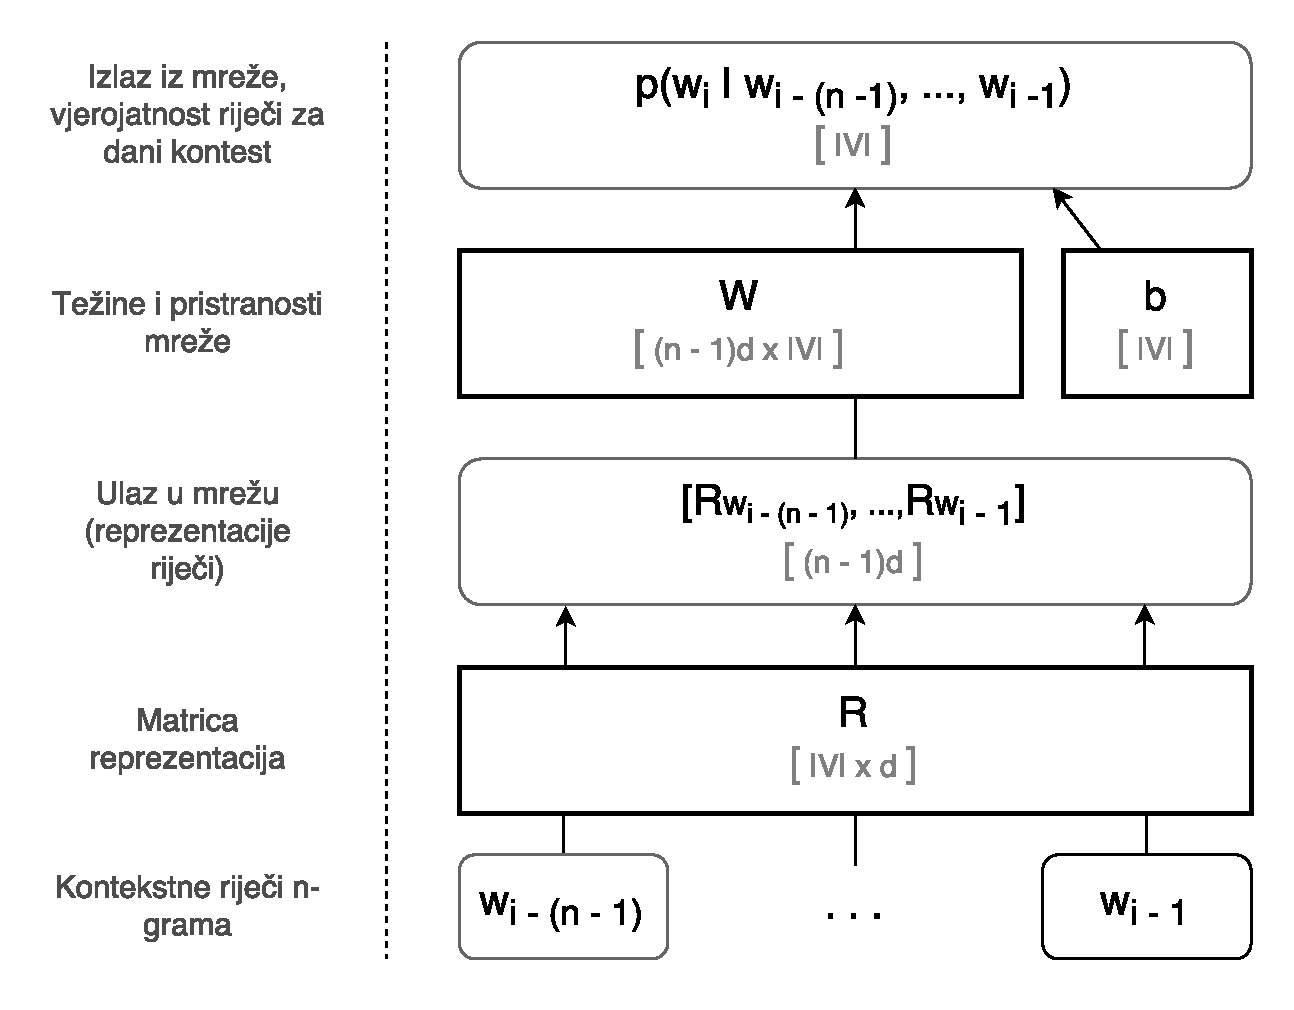
\includegraphics{fig/nnet.pdf}
\caption{Arhitektura neuronskog jezičnog modela. Pravokutnici s debljim rubovima su parametri mreže. Pravokutnici sa zaobljenim rubovima su podatci koji kroz mrežu prolaze.}
\label{fig:nnet}
\end{figure}

Može se primjetiti kako se za sve ulazne riječi koristi ista matrica distribuiranih vektora. Time se smanjuje broj parametara mreže i pospješuje učenje reprezentacija (riječi sličnog značenja dobivaju slične reprezentacije).

\section{Učenje}

Mreža korištena kao model jezika tipična je unaprijedna slojevita neuronska mreža. Mreže tog tipa treniraju se korištenjem \textit{"backpropagation"} algoritma. Gradijentnim spustom se smanjuje greška na skupu za treniranje. Osnove gradijentne optimizacije i \textit{"backpropagation"} algoritma neće biti opisane u ovom radu. Informacije na tu temu su široko dostupne, primjerice u CITAT - Čupić NENR.

Eventualna specifičnost neuronskog modela jezika, u odnosu na standardne unaprijedne slojevite mreže, je korištenje matrice reprezentacija $R$. Odabir retka matrice (što čini funkcija $d(...)$) nije standardna derivabilana matematička operacija. U tom smislu može se postaviti pitanje kako matricu $R$ optimirati gradijentnim spustom. Rješenje leži u tome da se matrica zapravo ne optimira u cjelosti, već se pri svakom podešavanju parametara mreže tijekom rada \textit{"backpropagation"} algoritma mjenjaju vrijednosti onih distribuiranih reprezentacija koje su u tom koraku korištene. Konkretno, reprezentacija riječi koje su bile na ulazu u mrežu.

\subsection{Gradijentna optimizacija}

Algoritam \textit{"backpropagation"} bazira se na gradijentnom spustu s obzirom na funkciju greške mreže. U originalu se greška minimizirala iterativno koristeći gradijent izračunat na cijelom skupu za učenje. U praksi se pokazalo kako je efikasnije podijeliti skup za učenje na manje grupe \engl{minibatch} i koristiti njih za gradijentni spust. Ekstrem ovog pristupa je podešavanje parametara mreže nakon evaluacije samo jednog primjera za učenje, što se naziva \textit{"online"} učenje. Ovaj ekstremni pristup rezultira nestabilnim gradijentom, zbog čega se mora smanjiti stopa učenja, i manjom efikasnošću korištenja računalnih resursa uslijed otežane paralelizacije. Stoga se najčešće koriste \textit{"minibatchevi"}. Konkretna veličina \textit{"minibatcha"} ovisi domeni primjene, arhitekturi mreže i načinu učenja. Ne postoji univerzalno prikladna veličina.

Osim "običnog" gradijentnog spusta, postoje i modificirane inačice. One parametre mreže ne mjenjaju samo izravno za veličinu negativnog gradijenta pomnoženog stopom učenja, već gradijent ili stopu učenja modificiraju. Najjednostavniji primjer modifikacije gradijenta je korištenje "momenta", pri čemu se čuva informacija o prethodnim iznosima gradijenta, akumulirana u "moment" (analogno momentu kretanja kuglice određene mase koja se kotrlja u smjeru nagiba, ali i u smjeru trenutne brzine). Postoje mnoge inačice gradijentnog spusta. U ovom radu korištena je inačica "RMSprop" \engl{resilient mean square propagation}, opisana u CITAT.

\section{Složenost mreže}

Pri izgradnji jezičnog modela potrebno je voditi račun o memorijskoj i vremenskoj složenosti izrade modela zbog veličine vokabulara koji se u jeziku koristi. U neuronskim mrežama je složenost treniranja usko vezana uz broj slobodnih parametara mreže. Stoga je potrebno vidjeti u kakvoj su vezi parametri jezičnog modela i neuronske mreže.

Matrica distribuiranih reprezentacija $R$ sadrži $|V| d$ parametara, matrica težina $W$ sadrži $(n - 1) d |V|$ parametara, a vektor pristranosti $|V|$ parametara. Sveukupno, mreža sadrži $(n d + 1) |V|$ parametara. Njena memorijska složenost stoga je $O(n d |V|)$. Vremenska složenost treniranja neuronske mreže ovisi o mnogim čimbenicima, ali se u ovom slučaju zbog jednostavnosti mreže može aproksimirati kao $O(n d |V|)$.

\section{Implementacija}

Za implementacije neuronskih mreža dostupni su mnogi alati. Većina njih je visoko optimizirana kako bi što učinkovitije koristili dostupne računalne resurse. Višeprocesorska i višejezgrena računala koriste se za paralelizaciju treniranja mreže, a sve dostupnija je i podrška za treniranje mreža koristeći visoki stupanj paralelizma grafičkih procesora. Nadalje, alati često podržavaju definiciju mreže na visokom stupnju apstrakcije i automatizirani izračun gradijenata, što olakšava implementaciju i smanjuje količinu grešaka u programskom kodu.

U ovom radu za korištena je \textit{open-source} knjižnica Theano\footnote{http://deeplearning.net/software/theano/}, čije sučelje je dostupno za jezik Python\footnote{https://www.python.org/}. Odabrana je zbog fleksibilnosti definiranja modela (lako se koristi s visoke razine apstrakcije, ali omogućava i rad na nižim razinama), automatiziranog izračuna gradijenata i mogućnosti izvršvanja istog koda na centralnim i grafičkim procesorima.

\chapter{Log-bilinearni model}

U radu CITAT 3-new-models-Mnih predložene su tri implementacije jezičnih modela. Najuspješniji među njima je log-bilinearni model koji se stoga evaluira u ovom radu.

Log-linearni prediktivni modeli CITAT su klasa modela u kojima je vjerojatnost uzorka proporcionalna eksponenciranoj linearnoj funkciji. Jednostavan primjer takvog modela je već korištena \textit{softmax} funkcija. Prikladni su za modeliranje vjerojatnosti jer eksponencijalna funkcija preslikava iz domene $\mathbb{R}$ u domenu $\mathbb{R}_{\leq 0}$, koja se lako normalizira u vjerojatnosni prostor. Istovremeno, logaritmiranje takve funkcije rezultira linearnom funkcijom (otkud ime "log-linearni modeli"), koja je pogodna za analizu i optimizaciju. Više informacija na temu log-linearnih modela može se naći u literaturi iz područja strojnog učenja CITAT.

Bilinearna funkcija je funkcija dvije varijable koja je s obzirom na njih obje linearna CITAT. Log-bilinearni model korišten u CITAT definira da je vjerojatnost proporcionalna eksponenciranoj bilinearnoj funkciji.

\[
P(a, b) \propto \exp(f_{lin}(a, b))
\]

\section{Log-bilinearni jezični model}

Log-bilinearna funkcija može se primjeniti za definiciju uvjetne vjerojatnosti riječi u jezičnom modelu s obzirom na kontekst. Razmatranja o načinu predstavljanja riječi iz poglavlja \ref{sec:lnnet_input} o neuronskom jezičnom modelu vrijede i za log-bilinearni model. Stoga se i u ovom modelu koriste distribuirane reprezentacije. Za kontekst definiran preko \textit{n}-grama, kakav je i dosad korišten u ovom radu, uvjetna vjerojatnost riječi ima sljedeći oblik.

\begin{equation}
P(w_i | w_{i - (n - 1)}, ... , w_{i - 1}) 
  \propto \exp(d(w_{i - (n - 1)}, ... , w_{i - 1}) W d(w_i)^T + b_{w_i})
\end{equation}

Funkcija $d(...)$ definirana je izrazom \ref{eq:d_func}. $W$ označava matricu preslikavanja $(n - 1)$ $d$-dimenzionalne reprezentacije na ulazu u jedan $d$-dimenzionalni vektor. Nakon što je time ulazni vektor reprezentacija reduciran na $d$ dimenzija, računa se skalarni produkt s reprezentacijom uvjetovan riječi, te se dodaje pristranost za tu riječ. Dobiveni rezultat potrebno je normalizirati u distribuciju vjerojatnosti nad svim riječima vokabulara.

\begin{equation}
P(w_i | w_{i - (n - 1)}, ... , w_{i - 1}) 
  = \frac{\exp(d(w_{i - (n - 1)}, ... , w_{i - 1}) W d(w_i)^T + b_{w_i})}
  {\sum_{w \in V} \exp(d(w_{i - (n - 1)}, ... , w_{i - 1}) W d(w)^T + b_{w})}
\end{equation}

Iako je ova definicija vrlo slična matematičkoj definiciji neuronskog modela jezika \ref{eq:lnnet}

\section{Učenje}

\section{Implementacija}

\chapter{Faktorizirani RBM}

\chapter{Evaluacija}

\section{Korpus}

\section{Metodologija}

\section{Mjera uspješnosti jezičnog modela}

\section{Rezultati}

\chapter{Zaključak} 

\bibliography{literatura}
\bibliographystyle{fer}

\chapter{Sažetak}

\end{document}
